%%%%%%%%%%%%%%%%%%%%%%%%%%%%%%%%%%%%%%%%%%%%%%%%%%%%%%%%%%%%%
% Article for the RBCA Journal                              %
% Supervised Classification of Clustering-Derived           %
% Employee Profiles: A People Analytics Study at ApexBrasil %
%%%%%%%%%%%%%%%%%%%%%%%%%%%%%%%%%%%%%%%%%%%%%%%%%%%%%%%%%%%%%

\documentclass[alpha-refs,english]{RBCA_v3.0}

% Uncomment this line if the article is in Portuguese.
%\AtBeginDocument{\renewcommand{\harvardand}{e}}

%%% Additional packages
\usepackage{booktabs}
\usepackage{multirow}
\usepackage{amsmath}
\usepackage{amssymb}
\usepackage{float}

%%% Paper title (English)
\title{Supervised Classification of Clustering-Derived Employee Profiles: A People Analytics Study at ApexBrasil}

%%% Portuguese title (mandatory if the paper is in Portuguese; optional here for bilingual papers)
\titleother{Classifica\c{c}\~ao Supervisionada de Perfis de Empregados Derivados de Clusteriza\c{c}\~ao: Um Estudo de People Analytics na ApexBrasil}

%%% Authors (anonymized for blind review; replace with author data when submitting final version)
\author[1]{C\'esar A. C. Moreira \orcid{0009-0001-0248-6791}}
\author[1]{Gladston Luiz da Silva \orcid{0000-0001-9650-2993}}

\affil[1]{Programa de P\'os-Gradua\c{c}\~ao em Computa\c{c}\~ao Aplicada, Universidade de Bras\'ilia (PPCA/UnB), Bras\'ilia, DF, Brazil}

%%% Author e-mails
\authnote{\authfn{1}cesar.moreira@aluno.unb.br; cesar.moreira@apexbrasil.com.br; gladston@unb.br}

%%% "Short" author for running page header
\runningauthor{Moreira and Silva}

%%% Paper category
\papercat{Original Paper}

%%% Editor fields - to be filled by RBCA editor
\jvolume{XX}
\jissue{X}
\jyear{2026}
\jmonth{Month}

\setcounter{page}{1}
\firstpage{1}
\jid{XXXX}

\jrec{yyyy-mm-dd}
\jrev{yyyy-mm-dd}
\jacc{yyyy-mm-dd}


\begin{document}

\begin{frontmatter}

\maketitle
\thispagestyle{empty}

\begin{Abstract}
This study represents Phase~2 of a People Analytics research program at ApexBrasil, the Brazilian Trade and Investment Promotion Agency. Building on Phase~1, which identified eight employee profiles through unsupervised clustering (K-Means, Silhouette Index = 0.34), this work evaluates four supervised classification models - Multinomial Logistic Regression, Decision Tree, Random Forest, and K-Nearest Neighbors (KNN) - for the operational assignment of new employees to the previously identified profiles. Because the target labels were generated by K-Means from the same feature space used as predictors, classification performance is interpreted as \textit{internal validation of the geometric separability of the Phase~1 profiles}, rather than as an external predictive assessment. Using anonymized data from 335 employees (2019--2023), with 70/30 train-test split and 10-fold stratified cross-validation, Multinomial Logistic Regression (accuracy: 0.96; 95\% CI: [0.92, 0.98]) and Random Forest (accuracy: 0.96) significantly outperform the remaining models (Cochran's Q = 175.97; p~$<$~0.001). The high accuracy confirms that the eight profiles are geometrically well separated in the feature space and demonstrates the operational feasibility of their automated assignment at the point of hiring.
\end{Abstract}

\begin{keywords}
CRISP-DM; Multinomial Logistic Regression; People Analytics; Random Forest; Supervised Classification
\end{keywords}

\begin{resumo}
Este estudo representa a Fase~2 de um programa de pesquisa em People Analytics na ApexBrasil, a Ag\^encia Brasileira de Promo\c{c}\~ao de Exporta\c{c}\~oes e Investimentos. Tendo como base a Fase~1, que identificou oito perfis de empregados por meio de clusteriza\c{c}\~ao n\~ao supervisionada (K-Means, \'Indice de Silhueta = 0,34), este trabalho avalia quatro modelos de classifica\c{c}\~ao supervisionada - Regress\~ao Log\'istica Multinomial, \'Arvore de Decis\~ao, Random Forest e K-Nearest Neighbors (KNN) - para a aloca\c{c}\~ao operacional de novos empregados aos perfis previamente identificados. Como os r\'otulos-alvo foram gerados pelo K-Means a partir do mesmo conjunto de atributos utilizado como preditor, o desempenho dos classificadores \'e interpretado como \textit{valida\c{c}\~ao interna da separabilidade geom\'etrica dos perfis da Fase~1}, e n\~ao como avalia\c{c}\~ao preditiva externa. Utilizando dados anonimizados de 335 empregados (2019--2023), com divis\~ao 70/30 treino-teste e valida\c{c}\~ao cruzada estratificada de 10 folds, a Regress\~ao Log\'istica Multinomial (acur\'acia: 0,96; IC 95\%: [0,92; 0,98]) e o Random Forest (acur\'acia: 0,96) superam significativamente os demais modelos (Q de Cochran = 175,97; p~$<$~0,001). A alta acur\'acia confirma que os oito perfis s\~ao geometricamente bem separados no espa\c{c}o de atributos e demonstra a viabilidade operacional de sua aloca\c{c}\~ao automatizada no momento da contrata\c{c}\~ao.
\end{resumo}

\begin{palavras_chave}
Classifica\c{c}\~ao Supervisionada; CRISP-DM; People Analytics; Random Forest; Regress\~ao Log\'istica Multinomial
\end{palavras_chave}

\end{frontmatter}


\section{Introduction}
People Analytics refers to the application of data science techniques to human resource processes, enabling data-driven workforce decision-making and reshaping organizational talent management practices \citep{Ferrar2021,Margherita2022}. In a constantly changing organizational environment, the ability to predict employee behaviors and allocate individuals to appropriate workforce segments is a strategic capability for organizations navigating rapid socio-economic transformations \citep{Polzer2022}.

In Phase~1 of this research program \citep{Moreira2026}, unsupervised clustering techniques were applied to employee data at ApexBrasil - the Brazilian Trade and Investment Promotion Agency - identifying eight distinct workforce profiles through K-Means (Silhouette Index = 0.34, 100\% sample coverage). The resulting segments, characterized by combinations of age, gender, Hired Time, dependents, and absenteeism patterns, provide an interpretable basis for differentiated people management policies.

However, segmentation alone is insufficient for operational implementation. Each time a new employee joins the organization, there is a practical need to assign them to the appropriate profile based on their individual attributes. This requires supervised classification models trained on the cluster labels discovered in Phase~1. Classification is a supervised machine learning technique used to predict the category to which a new observation belongs, based on a training dataset containing observations whose categories are known \citep{Han2012}.

The classification of employees in the context of Human Resources must be applied with due caution, considering the ethical implications of labeling individuals. Models should serve to identify situations in which individual well-being and performance can be improved, not to create discriminatory practices \citep{Tursunbayeva2022}.

Given this context, the central research question guiding this study is: \textit{``Which supervised classification techniques most faithfully recover the geometric structure of employee profiles derived from unsupervised clustering, enabling their operational assignment in a Brazilian public organization with limited analytical maturity?''}

This question unfolds into three specific research questions: (i)~Which classification models most faithfully recover the geometric boundaries of the eight workforce profiles identified in Phase~1? (ii)~How do model performances compare across established evaluation metrics and statistical tests? (iii)~What implications do the results have for the operational assignment of new employees to these profiles in organizational settings?

ApexBrasil is a federal public organization linked to the Ministry of Development, Industry, Commerce and Services (MDIC), operating in commercial promotion and foreign investment attraction. Relevant organizational characteristics include approximately 335 employees under Brazilian Labor Law (CLT) regime, an integrated TOTVS ERP system, and an initial stage of analytics adoption. The organization was selected based on data availability, analytical relevance, and alignment with an ongoing people management modernization initiative, as detailed in Phase~1 \citep{Moreira2026}.

\subsection{General Objective} 

To evaluate and compare supervised classification techniques (Multinomial Logistic Regression, Decision Tree, Random Forest, and K-Nearest Neighbors) for the operational assignment of new employees to workforce profiles previously identified through clustering at ApexBrasil, treating classification performance as internal validation of the geometric separability of these profiles rather than as external predictive assessment.

\subsection{Specific Objectives} 

\begin{enumerate}
    \item Employ the eight workforce profiles from Phase~1 as target labels for supervised classification.
    \item Implement and compare four classification models using the same demographic, temporal, and absenteeism attributes from Phase 1. 
    \item Evaluate model performance through Accuracy, Precision, Recall, F1-Score, ROC Curve analysis, confidence intervals, and statistical hypothesis tests.
    \item Assess the feasibility and implications of automated employee classification for organizational HR management.
\end{enumerate}

\subsection{Scientific contributions} This study contributes in three dimensions: 
\begin{enumerate}
    \item \textbf{Theoretical}: validates the sequential CRISP-DM approach (clustering~$\rightarrow$~classification) for People Analytics in the Brazilian public sector, demonstrating that the Phase~1 profiles exhibit sufficient geometric separability in the feature space to be reliably recovered by supervised models, which in turn operationalizes their automated assignment to new employees.
    \item \textbf{Methodological}: provides a replicable protocol with rigorous statistical validation (10-fold CV, confidence intervals, Cochran's Q, McNemar pairwise tests) for evaluating classification techniques applied to clustering-derived labels.
    \item \textbf{Practical}: demonstrates the feasibility of automating employee profile assignment at the point of hiring, offering an operational pathway for organizations with low analytical maturity.
\end{enumerate}

The remainder of this article is organized as follows: \cref{sec:framework} presents the theoretical framework on supervised classification techniques; \cref{sec:methodology} details the methodology; \cref{sec:results} presents results; \cref{sec:discussion} discusses findings and their implications; and \cref{sec:conclusions} concludes with contributions, limitations, and directions for future research.


\section{Theoretical Framework}
\label{sec:framework}

From Segmentation to Classification: The Phase 1--Phase 2 Continuum
Clustering and classification are complementary but distinct analytical approaches. Clustering (unsupervised learning) discovers natural groups in data without prior labels, while classification (supervised learning) predicts membership in known categories \citep{Rokach2005}. In People Analytics applications, a sequential approach is particularly powerful: clustering first identifies workforce segments, then classification enables operational deployment by predicting segment membership for new observations \citep{Edwards2019,Garg2022}.

Phase~1 of this research \citep{Moreira2026} applied three clustering techniques (K-Means, Hierarchical Clustering, and DBSCAN) to ApexBrasil's employee data, selecting K-Means with $k=8$ as the optimal solution based on dual criteria of technical quality (Silhouette Index = 0.34) and organizational utility (100\% sample coverage). The eight resulting profiles - ranging from young entry-level employees to pre-retirement high-compensation workers - constitute the target variable for the present classification study.

This Phase~1--Phase~2 continuum aligns with the analytical maturity progression described by \cite{Lismont2017}, where organizations evolve from descriptive analytics (segmentation) to predictive analytics (classification and forecasting).

\subsection{Classification Models}
The four classification models evaluated in this study are presented below 
with their canonical formulations.

\subsubsection{Multinomial Logistic Regression}
Multinomial Logistic Regression extends binary logistic regression to 
multiclass problems by modeling the probability of each of $K$ classes 
relative to a reference class \citep{Hosmer2013,Cox1958,Menard2008}:

\begin{equation}
P(Y=k \mid X) = \frac{\exp(\beta_k \cdot X)}{\sum_{j=1}^{K} \exp(\beta_j \cdot X)}
\label{eq:multinom}
\end{equation}

\subsubsection{Decision Trees}
Decision Trees segment data into homogeneous regions through recursive 
partitioning, with node impurity measured by entropy or the Gini index 
\citep{Breiman2017,Quinlan1986,Safavian1991}:

\begin{equation}
Gini(t) = 1 - \sum_{i=1}^{K} p(i \mid t)^2
\label{eq:gini}
\end{equation}

\noindent where $p(i \mid t)$ is the proportion of class $i$ observations in 
node $t$. The index reaches 0 when the node is pure.

\subsubsection{Random Forest}
Random Forest is an ensemble combining multiple decision trees, aggregating 
predictions via majority voting \citep{Breiman2001,Cutler2007}:

\begin{equation}
\hat{y} = \mathrm{mode}\{h_1(x), h_2(x), \ldots, h_B(x)\}
\label{eq:rf}
\end{equation}

\noindent where $h_b(x)$ is the prediction of the $b$-th of $B$ trees.

\subsubsection{K-Nearest Neighbors (KNN)}
KNN classifies a new observation by majority vote among its $k$ nearest 
neighbors in feature space \citep{Cover1967,Altman1992,Duda2001}:

\begin{equation}
\hat{y} = \arg\max_{c} \sum_{x_i \in N_k(x)} \mathbb{I}(y_i = c)
\label{eq:knn}
\end{equation}

\noindent where $N_k(x)$ is the set of $k$ nearest neighbors of $x$ and 
$\mathbb{I}(\cdot)$ is the indicator function.

\subsection{Related Works}
\cite{Garg2022} presented a systematic literature review identifying that Machine Learning applications in HR are strongest in recruitment and performance management, with decision trees and classification algorithms dominating across HR functions. \cite{Alsaadi2022} applied Logistic Regression, Decision Tree, and Random Forest comparatively to HR practices, using Precision and Accuracy as success metrics. \cite{Liao2023} compared classification models for employee turnover prediction. \cite{Padmaja2022} conducted experiments with classification algorithms including Logistic Regression, KNN, Decision Tree, Random Forest, and AdaBoost to analyze performance metrics. \cite{Lawrance2021} used classification methods to assess the cost of absenteeism and define metrics to support decision-making. \cite{Fallucchi2020} proposed an analysis comparing Accuracy, Precision, Recall, and F1-Score, achieving success in predicting employee turnover.

These studies apply classification to HR data but typically use externally defined target variables (e.g., ``attrited'' vs. ``retained''). The present study extends this literature by applying classification to internally derived clustering labels, explicitly connecting unsupervised segmentation with supervised prediction in a sequential analytical framework, and introducing rigorous statistical hypothesis testing for model comparison.


\section{Methodology}
\label{sec:methodology}

This study follows the CRISP-DM framework \citep{Chapman2000}, continuing from Phase~1 \citep{Moreira2026}, which covered Business Understanding, Data Understanding, and initial Modeling (clustering). Phase~2 focuses on: (1)~Modeling supervised classifiers; and (2)~Evaluating classification performance with statistical rigor.

\subsection{Dataset and Target Variable}
The dataset is identical to Phase~1: anonymized data from 335 active employees at ApexBrasil, extracted from the TOTVS ERP system, covering the period January 2019 to December 2023. Data extraction, transformation, loading (ETL), and exploratory analysis are detailed in Phase~1 \citep{Moreira2026}.

\begin{table}[H]
    \centering
    \resizebox{\columnwidth}{!}{%
    \begin{threeparttable}
    \caption{Variables Used in Classification}
    \label{tab:variables}
    \begin{tabular}{llll}
        \toprule
        Variable & Type & Description & Unit \\
        \midrule
        Age (IDADE) & Numeric & Employee age & Years \\
        Dependents (TOTAL\_DEPENDENTES) & Numeric & Number of dependents & Count \\
        Hired Time (TEMPO\_DE\_CASA) & Numeric & Length of service & Years \\
        Absenteeism (TOTAL\_MINUTOS) & Numeric & Total absence time & Minutes \\
        Gender (GENERO) & Categorical & Male (2) / Female (1) & - \\
        \bottomrule
    \end{tabular}
    \begin{tablenotes}
        \footnotesize
        \item Source: TOTVS ERP system, ApexBrasil \citep{Moreira2026}.
    \end{tablenotes}
    \end{threeparttable}%
    }
\end{table}

Target variable: The eight workforce profiles identified in Phase~1 via K-Means clustering ($k=8$, Silhouette Index = 0.34, 100\% sample coverage). Each of the 335 employees carries a cluster label (1 through 8) assigned during Phase~1 segmentation. \cref{tab:distribution} presents the distribution.

\begin{table*}[!b]
    \centering
    \begin{threeparttable}
    \caption{Distribution of Employees Across Cluster-Derived Classes}
    \label{tab:distribution}
    \begin{tabularx}{\textwidth}{cccccccc>{\raggedright\arraybackslash}X}
        \toprule
        Cluster & N & \% & Age ($\mu$) & Hired Time ($\mu$) & Dep. ($\mu$) & Absent. h ($\mu$) & \% Female & Profile Description \\
        \midrule
        1 & 22  & 6.6  & 61 & 3  & 0.0 & 99    & 23  & Senior, recently hired, predominantly male \\
        2 & 51  & 15.2 & 47 & 14 & 0.2 & 155   & 0   & Experienced, long-tenured, male, low dependents \\
        3 & 34  & 10.1 & 44 & 11 & 3.0 & 260   & 100 & Mature women, high dependents, high absenteeism \\
        4 & 77  & 23.0 & 34 & 4  & 0.4 & 146   & 0   & Young males, early career \\
        5 & 15  & 4.5  & 41 & 10 & 1.0 & 1{,}327 & 73  & Mixed gender, extreme absenteeism \\
        6 & 58  & 17.3 & 36 & 4  & 0.3 & 184   & 100 & Young women, early career \\
        7 & 48  & 14.3 & 48 & 13 & 0.3 & 247   & 100 & Senior women, long-tenured \\
        8 & 30  & 9.0  & 50 & 13 & 2.9 & 169   & 0   & Mature males, long-tenured, high dependents \\
        \midrule
        Total & 335 & 100 & & & & & & \\
        \bottomrule
    \end{tabularx}
    \begin{tablenotes}
        \footnotesize
        \item Source: Phase~1 results \citep{Moreira2026}.
    \end{tablenotes}
    \end{threeparttable}
\end{table*}

\subsection{Classification Approach}

\subsubsection{Why High Accuracy Is Expected}
\label{sec:why_high}
An important epistemological consideration shapes the interpretation of the results that follow: the target variable (cluster labels) was generated by K-Means from the same feature set used as predictors in the supervised stage. Consequently, the supervised models are not learning to predict an externally defined outcome but rather to \textit{reconstruct the K-Means partitioning decision} in the feature space. High classification accuracy is therefore an expected consequence of the sequential design, not a measure of external predictive validity in the sense classically employed in supervised learning \citep{Hastie2009}.

This design is best understood as a form of \textbf{internal validation of cluster separability} rather than as predictive assessment against independent ground truth. The literature on cluster validity recognizes this distinction: when ``true clusters'' are not externally observable, supervised recovery from the same features constitutes evidence of geometric separability - that is, evidence that the groups discovered by the unsupervised algorithm occupy sufficiently distinct regions of the feature space to be consistently delineated by alternative learners \citep{Hennig2015}. Accordingly, the classification experiment reported here serves two legitimate purposes: (i)~to validate that the Phase~1 segmentation represents well-defined, geometrically separable groups rather than algorithmic artifacts, and (ii)~to \emph{operationalize} the assignment of new employees to these groups, replacing re-execution of the clustering algorithm with a trained classifier at the point of hiring. Both purposes are internal to the organization's data environment and do not, by themselves, establish that the profiles would generalize as predictive categories to other organizations or future workforce configurations. The diagnostic value of inter-model comparison is preserved under this framing: low accuracy for certain models (e.g., KNN) still provides substantive information about model-data fit and the geometric properties of cluster boundaries, as elaborated in \cref{sec:knn_optimization}.

\subsubsection{Train-Test Split and Cross-Validation}
The dataset was divided into 70\% for training ($n=234$) and 30\% for testing ($n=101$) using stratified sampling to preserve class proportions. Model performance was evaluated using \textbf{10-fold stratified cross-validation} on the training set, with a fixed random seed (seed = 123) ensuring full reproducibility.

Cross-validation configuration: 10 folds (stratified); 1 repetition; seed = 123; train partition 70\% ($n=234$); test partition 30\% ($n=101$).

\subsubsection{Computational Environment}
All analyses were performed in Python 3.12 using scikit-learn 1.8.0. For Multinomial Logistic Regression, the Newton-CG solver was employed (equivalent to R's \texttt{nnet::multinom} Newton-Raphson optimizer). Random Forest used 500 trees. KNN's optimal $k$ was determined via cross-validation grid search ($k=1$ to $20$). Processing was performed with a fixed random seed (123) across all stochastic components.

\subsection{Evaluation Metrics}
Model performance was evaluated using four complementary metrics \citep{Sokolova2009,VanRijsbergen1979}, calculated per class and reported as weighted averages:

\begin{itemize}
    \item \textbf{Accuracy}: measures the overall proportion of correctly classified observations.
\end{itemize}

\begin{equation}
\mathrm{Accuracy} = \frac{TP + TN}{TP + TN + FP + FN}
\label{eq:accuracy}
\end{equation}

\noindent where $TP$ denotes true positives, $TN$ true negatives, $FP$ false positives, and $FN$ false negatives.

\begin{itemize}
    \item \textbf{Precision}: quantifies the proportion of correctly predicted positive observations among all observations predicted as positive.
\end{itemize}

\begin{equation}
\mathrm{Precision} = \frac{TP}{TP + FP}
\label{eq:precision}
\end{equation}

Precision reflects the reliability of positive predictions and penalizes false positives.

\begin{itemize}
    \item \textbf{Recall (Sensitivity)}: also known as sensitivity, measures the proportion of actual positive observations correctly identified by the model.
\end{itemize}

\begin{equation}
\mathrm{Recall} = \frac{TP}{TP + FN}
\label{eq:recall}
\end{equation}

Recall emphasizes the model's ability to detect true positive cases and penalizes false negatives.

\begin{itemize}
    \item \textbf{F1-Score}: represents the harmonic mean of Precision and Recall \citep{Christen2024}, balancing both metrics into a single performance indicator.
\end{itemize}

\begin{equation}
\mathrm{F1} = 2 \times \frac{\mathrm{Precision} \times \mathrm{Recall}}{\mathrm{Precision} + \mathrm{Recall}}
\label{eq:f1}
\end{equation}

The F1-score is particularly useful in contexts with class imbalance, as it penalizes extreme values in either precision or recall.

\textbf{Confidence intervals} (95\%) were computed using the $t$-distribution across cross-validation folds. For paired model comparisons, the \cite{Nadeau2003} variance correction was applied. Given the small number of folds ($k=10$), degrees of freedom were defined as $df = k - 1 = 9$. The confidence interval for each metric was calculated as:

\begin{equation}
\bar{x} \pm t_{0.975,\,9} \cdot \frac{s}{\sqrt{k}}
\label{eq:ci}
\end{equation}

\noindent where $\bar{x}$ is the mean metric across folds, $s$ is the standard deviation across folds, $k = 10$ folds, and $t_{0.975,\,9} \approx 2.262$.

\subsection{Statistical Hypothesis Tests}
Three complementary statistical tests were applied to compare model performance:

\begin{itemize}
    \item \textbf{Cochran's Q test} (omnibus): Tests whether all models have the same error rate on the test set. $H_0$: all models perform equally; $H_1$: at least one model differs. The test statistic follows a $\chi^2$ distribution with $df = k - 1$ \citep{Cochran1950}.
    \item \textbf{McNemar's test} (pairwise): Tests whether two specific models differ in their error patterns on the same test set, using the $2 \times 2$ contingency of discordant predictions. Bonferroni correction was applied for 6 pairwise comparisons ($\alpha_{corrected} = 0.05/6 = 0.0083$) \citep{McNemar1947}.
    \item \textbf{Corrected paired t-test} (pairwise): Compares cross-validation fold accuracies between model pairs. The \cite{Nadeau2003} correction was applied to account for the non-independence of training sets across folds, adjusting the variance estimate by the test-to-training ratio.
\end{itemize}

\subsection{ROC Curve Analysis}
Receiver Operating Characteristic (ROC) curves \citep{Fawcett2006} were generated for all models supporting probability estimates. For the multiclass setting (8 classes), a one-vs-all strategy was applied: each class was treated as positive against all others. Macro-averaged ROC curves were computed by interpolating per-class curves onto a common false positive rate grid and averaging true positive rates. Area Under the Curve (AUC) was computed per class and averaged.


\section{Results}
\label{sec:results}

\subsection{Correlation Analysis}
\cref{tab:correlation} presents the correlation matrix for numerical variables. The strongest correlation ($r = 0.41$) occurs between Age and Hired Time, classified as \textbf{moderate} according to \cite{Cohen2013}, where strong correlation requires $r > 0.70$. No multicollinearity concerns are present.

\begin{table}[H]
    \centering
    \begin{threeparttable}
    \caption{Correlation Matrix}
    \label{tab:correlation}
    \begin{tabularx}{\columnwidth}{l*{4}{>{\centering\arraybackslash}X}}
        \toprule
         & Age & H.T. & Dep. & Absent. \\
        \midrule
        Age              & 1.000 & 0.413 & 0.121 & 0.011 \\
        H.T.           & 0.413 & 1.000 & 0.282 & 0.166 \\
        Dep.             & 0.121 & 0.282 & 1.000 & 0.161 \\
        Absent.          & 0.011 & 0.166 & 0.161 & 1.000 \\
        \bottomrule
    \end{tabularx}
    \begin{tablenotes}
        \footnotesize
        \item H.T. = Hired Time; Dep. = Dependents; Absent. = Absenteeism (h).
        \item Source: Elaborated by the author.
    \end{tablenotes}
    \end{threeparttable}
\end{table}

\cref{tab:correlation} reveals low-to-moderate associations among predictors. 
The strongest correlation - between Age and Hired Time ($r = 0.413$) - is 
substantively expected in a stable public-sector workforce, but explains only 
17\% of shared variance, preserving the discriminative independence of both 
variables. Hired Time and Dependents ($r = 0.282$) reflect life-cycle effects 
without rising to the level of redundancy. Absenteeism is weakly correlated 
with all other variables (max $r = 0.166$), constituting an independent 
behavioral dimension orthogonal to demographic attributes.

The absence of strong correlations ($r > 0.70$) has two methodological 
consequences: (i) Multinomial Logistic Regression coefficients are interpretable 
without multicollinearity-induced instability; and (ii) Random Forest variable 
importance rankings (\cref{fig:importance}) reflect genuine predictive 
contributions rather than artifacts of correlated inputs.

\subsection{Cross-Validation Results with Confidence Intervals}

\cref{tab:cv_metrics} consolidates cross-validation and held-out test 
performance for the four models, enabling distinction between estimated 
generalization (CV) and observed performance on unseen data (test).

For the three top models, test accuracy falls within or above the CV 
confidence interval (Multinomial LR: 0.949 CV vs. 0.960 test; Random Forest: 
0.910 vs. 0.960; Decision Tree: 0.859 vs. 0.941), providing strong evidence 
of stable generalization with no signs of overfitting. The Accuracy-F1 gap 
within each model is small (<1 percentage point for Multinomial LR), 
indicating balanced performance across minority and majority classes. The 
slightly larger gap for Random Forest (0.910 vs. 0.894) anticipates the 
Cluster 5 weakness detailed in \cref{tab:per_class_rf}.

KNN stands in categorical contrast: CV Accuracy of 0.300 [0.220, 0.380], 
Test Accuracy of 0.277, and the lowest F1-Score (0.261). The width of its 
CI (16 percentage points, more than double the top three) signals genuine 
instability rather than mere underperformance.

\begin{table*}[!t]
    \centering
    \begin{threeparttable}
    \caption{Classification Metrics with 95\% Confidence Intervals}
    \label{tab:cv_metrics}
    \begin{tabular}{lcccccc}
        \toprule
        Model & CV Accuracy & 95\% CI & CV F1 (wtd) & 95\% CI & Test Acc. & Test F1 \\
        \midrule
        \textbf{Multinomial Log. Reg.} & \textbf{0.9487} & \textbf{[0.917, 0.980]} & \textbf{0.9432} & \textbf{[0.907, 0.979]} & \textbf{0.9604} & \textbf{0.9615} \\
        Random Forest                  & 0.9101 & [0.876, 0.945] & 0.8940 & [0.856, 0.933] & 0.9604 & 0.9543 \\
        Decision Tree                  & 0.8591 & [0.816, 0.902] & 0.8457 & [0.798, 0.893] & 0.9406 & 0.9403 \\
        KNN ($k=13$)                   & 0.2998 & [0.220, 0.380] & 0.2608 & [0.187, 0.335] & 0.2772 & 0.2603 \\
        \bottomrule
    \end{tabular}
    \begin{tablenotes}
        \footnotesize
        \item Source: Elaborated by the author. CV = 10-fold CV, seed = 123.
    \end{tablenotes}
    \end{threeparttable}
\end{table*}

\begin{figure}[H]
    \centering
    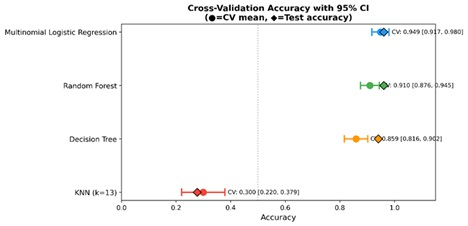
\includegraphics[width=\linewidth]{figures/fig_cv_accuracy.jpeg}
    \caption{Cross-validation accuracy with 95\% confidence intervals (circles) and held-out test accuracy (diamonds) for all four classification models. Source: Elaborated by the author.}
    \label{fig:cv_accuracy}
\end{figure}

\cref{fig:cv_accuracy} visualizes a striking \textbf{bimodal performance 
landscape}: three models cluster above 0.85 accuracy while KNN occupies an 
isolated region around 0.30 - a gap of more than 60 percentage points 
signaling a qualitative, not incremental, difference. Within the top cluster, 
Multinomial LR shows the narrowest CI (6.3 percentage points), followed by 
Random Forest (6.9 pp) and Decision Tree (8.6 pp) - a progression consistent 
with the inductive biases of each algorithm when applied to convex, 
centroid-based cluster boundaries.

\begin{figure}[H]
    \centering
    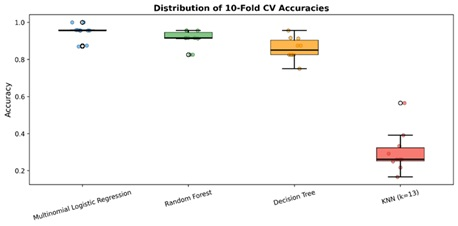
\includegraphics[width=\linewidth]{figures/fig_fold_distribution.jpeg}
    \caption{Distribution of per-fold accuracy across 10 cross-validation folds, showing median, interquartile range, and individual fold results. Source: Elaborated by the author.}
    \label{fig:fold_distribution}
\end{figure}

\cref{fig:fold_distribution} exposes the fold-by-fold variability obscured 
by aggregate CIs. Multinomial LR and Random Forest exhibit tight, symmetric 
distributions, confirming that their high accuracy is not driven by a few 
favorable folds. Decision Tree shows slightly more dispersion with a longer 
lower whisker - a known behavior of single trees on small samples. KNN's 
per-fold accuracies span a wide range below 0.30, with a distribution shape 
signaling instability rather than mere weakness: in dense regions of the 
feature space, the 13 nearest neighbors are informative; in sparse regions 
(notably Cluster 5 with $n=15$), they are dominated by majority classes from 
adjacent clusters, producing systematic misclassification. The pattern 
reflects a structural mismatch between KNN's locality assumption and the 
heterogeneous cluster densities of the dataset (cluster sizes range from 
$n=15$ to $n=77$).

Together, \cref{fig:cv_accuracy,fig:fold_distribution} establish that the 
top three models exhibit similar mean accuracy \emph{and} similar stability 
profiles - which is why formal hypothesis testing 
(\cref{tab:mcnemar,tab:ttests}) will fail to reject equivalence among them 
while strongly rejecting it for KNN.

\subsection{Confusion Matrices}
\label{sec:confusion}

Fig.~\ref{fig:confusion} presents the confusion matrices for all four 
models on the held-out test set.

\begin{figure*}[!t]
    \centering
    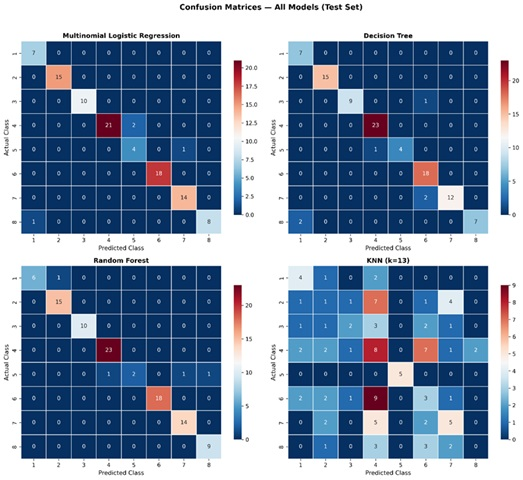
\includegraphics[width=\textwidth]{figures/fig_confusion_matrices.jpeg}
    \caption{Confusion matrices for the four classification models on the held-out test set ($n = 101$). Rows represent actual classes; columns, predicted classes. Diagonal cells show correct classifications. Source: Elaborated by the author.}
    \label{fig:confusion}
\end{figure*}

The confusion matrices corroborate the aggregate metrics in 
\cref{tab:cv_metrics}: Multinomial Logistic Regression and Random Forest 
concentrate predictions along the main diagonal, with off-diagonal errors 
confined to a small number of adjacent clusters - notably the boundary between 
Clusters 1 and 8 (mature males with long tenure) and isolated misclassifications 
in Cluster 5. Decision Tree exhibits a similar diagonal pattern with marginally 
more dispersion. KNN, in contrast, produces predictions widely scattered across 
the matrix, with systematic over-assignment to the larger clusters (notably 
Cluster 4) regardless of true class - a direct consequence of the 
neighborhood-density bias discussed in \cref{sec:knn_optimization}.

\subsection{Per-Class Metrics}

\cref{tab:per_class_lr,tab:per_class_rf} decompose the aggregate accuracy 
of 0.96 into class-specific metrics for the two best-performing models. 
Two models can reach identical aggregate accuracy through different error 
patterns - a distinction with direct operational consequences for 
differentiated HR policies.

Multinomial LR (\cref{tab:per_class_lr}) achieves perfect or near-perfect 
classification in five clusters (2, 3, 6 with F1 = 1.000; 4 and 7 with 
F1 > 0.95). The two clusters with imperfect performance are informative. 
Cluster 1 (precision 0.875, recall 1.000) shows a slightly over-inclusive 
decision boundary. Cluster 5 (precision 0.667, recall 0.800, F1 = 0.727) 
is the weakest overall, reflecting both small sample size ($n = 5$) and 
its location in a sparse region of feature space defined primarily by 
extreme absenteeism.

\begin{table}[ht]
    \centering
    \begin{threeparttable}
    \caption{Per-Class Metrics: Multinomial Logistic Regression}
    \label{tab:per_class_lr}
    \begin{tabular}{ccccc}
        \toprule
        Class & Precision & Recall & F1-Score & Support \\
        \midrule
        1            & 0.875 & 1.000 & 0.933 & 7 \\
        2            & 1.000 & 1.000 & 1.000 & 15 \\
        3            & 1.000 & 1.000 & 1.000 & 10 \\
        4            & 1.000 & 0.913 & 0.955 & 23 \\
        5            & 0.667 & 0.800 & 0.727 & 5 \\
        6            & 1.000 & 1.000 & 1.000 & 18 \\
        7            & 0.933 & 1.000 & 0.966 & 14 \\
        8            & 1.000 & 0.889 & 0.941 & 9 \\
        \midrule
        Weighted avg & 0.966 & 0.960 & 0.962 & 101 \\
        \bottomrule
    \end{tabular}
    \begin{tablenotes}
        \footnotesize
        \item Source: Elaborated by the author.
    \end{tablenotes}
    \end{threeparttable}
\end{table}

Random Forest (\cref{tab:per_class_rf}) produces a structurally different 
per-class profile despite the same aggregate accuracy. It achieves perfect 
classification in Clusters 3, 4, 6, and 7, but its Cluster 5 performance 
inverts LR's pattern: precision = 1.000 but recall = 0.400 (F1 = 0.571), 
meaning RF makes confident predictions when it identifies the class but 
misses 60\% of true instances. This asymmetry is illuminating: LR's 
continuous coefficients allow extreme absenteeism to push observations 
toward the correct prediction, while RF's majority voting de-prioritizes 
Absenteeism (Gini = 0.139; \cref{fig:importance}), causing Cluster 5 
instances to be absorbed into adjacent demographically similar clusters. 
The decoupling between high AUC (0.999; \cref{tab:auc}) and low recall 
(0.400) confirms that RF \emph{ranks} Cluster 5 correctly but its default 
threshold fails to convert that ranking into classification - a distinction 
relevant for threshold tuning at deployment.

\begin{table}[ht]
    \centering
    \begin{threeparttable}
    \caption{Per-Class Metrics: Random Forest}
    \label{tab:per_class_rf}
    \begin{tabular}{ccccc}
        \toprule
        Class & Precision & Recall & F1-Score & Support \\
        \midrule
        1            & 1.000 & 0.857 & 0.923 & 7 \\
        2            & 0.938 & 1.000 & 0.968 & 15 \\
        3            & 1.000 & 1.000 & 1.000 & 10 \\
        4            & 0.958 & 1.000 & 0.979 & 23 \\
        5            & 1.000 & 0.400 & 0.571 & 5 \\
        6            & 1.000 & 1.000 & 1.000 & 18 \\
        7            & 0.933 & 1.000 & 0.966 & 14 \\
        8            & 0.900 & 1.000 & 0.947 & 9 \\
        \midrule
        Weighted avg & 0.963 & 0.960 & 0.954 & 101 \\
        \bottomrule
    \end{tabular}
    \begin{tablenotes}
        \footnotesize
        \item Source: Elaborated by the author.
    \end{tablenotes}
    \end{threeparttable}
\end{table}

The two models also offer \textbf{complementary strengths} on boundary
clusters: Cluster 1 is handled better by RF (precision 1.000) than by LR
(0.875), while Cluster 2 is perfect for LR but slightly imperfect for RF
(precision 0.938); Cluster 8 shows the reverse pattern. This suggests that
a soft-voting ensemble of LR and RF probability outputs could plausibly
outperform either model individually on minority clusters - a direction
for future operational deployment beyond the scope of this study. From a
practical HR perspective, the high-confidence clusters (2, 3, 4, 6, 7)
account for 78\% of test observations, supporting a \textbf{tiered
deployment strategy}: automated classification for these clusters, with
manual HR review flagged for boundary (1, 8) and minority (5) clusters.

A methodological caveat accompanies these per-class metrics: the small
test-set support for Cluster 5 ($n=5$) and Cluster 1 ($n=7$) implies that
their precision and recall estimates carry wide intrinsic uncertainty
(single misclassifications produce 15--20 percentage-point swings). These
figures should therefore be interpreted as \textit{directional} rather
than definitive, and the tiered deployment strategy above is partly
motivated by this uncertainty.

\subsection{ROC Curve Analysis}

\cref{fig:roc} and \cref{tab:auc} present the comparative ROC analysis. The 
ROC framework is particularly valuable here because it evaluates models 
\textbf{independently of the classification threshold} and is insensitive to 
class imbalance, properties that aggregate accuracy lacks in multiclass 
settings with uneven class sizes ($n = 15$ to $n = 77$ in this study).

The macro-averaged curves in panel~(A) reveal three distinct performance 
tiers. Random Forest and Multinomial Logistic Regression both reach Mean 
AUC = 0.999, with standard deviations across classes of 0.001 and 0.002 - 
two orders of magnitude smaller than typical reporting precision, confirming 
that near-perfect ranking is achieved \emph{uniformly} across all eight 
clusters rather than driven by a few easy ones. Decision Tree forms a second 
tier (AUC = 0.954, Std = 0.041), with variability reflecting its discrete 
step-like probability outputs. KNN occupies a third tier near the diagonal 
of random performance (AUC = 0.668, Std = 0.172), confirming that its 
failure observed in the confusion matrices is not a threshold-tuning problem: 
at any operating point, KNN's rankings are barely better than chance.

The per-class curves in panel~(B) show all eight Random Forest cluster 
curves clustered near the optimal corner. Notably, Cluster 5 - identified 
in \cref{tab:per_class_rf} as RF's weak spot in absolute classification 
(recall = 0.400) - exhibits AUC near 1.0. This \textbf{decoupling between 
probability quality (AUC) and classification quality (recall)} indicates 
that the model's Cluster 5 problem stems from its default threshold 
(majority vote across trees) being too conservative for a minority class, 
not from poor probability calibration. Operationally, this suggests that 
threshold adjustment or class-weighted prediction rules could substantially 
improve recall on minority profiles without retraining - an important 
consideration for deployment in HR settings where minority profiles may 
require differentiated attention.

\begin{figure*}[!t]
    \centering
    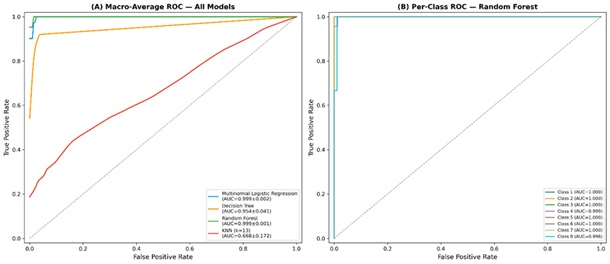
\includegraphics[width=.85\textwidth]{figures/fig_roc.jpeg}
    \caption{(A)~Macro-averaged ROC curves comparing all four models. (B)~Per-class ROC curves for Random Forest, demonstrating near-perfect discrimination across all eight clusters. Source: Elaborated by the author.}
    \label{fig:roc}
\end{figure*}

\begin{table}[ht]
    \centering
    \begin{threeparttable}
    \caption{Mean AUC by Model (Macro-Averaged)}
    \label{tab:auc}
    \begin{tabular}{lcc}
        \toprule
        Model & Mean AUC & Std \\
        \midrule
        Random Forest                   & 0.999 & 0.001 \\
        Multinomial Logistic Regression & 0.999 & 0.002 \\
        Decision Tree                   & 0.954 & 0.041 \\
        KNN ($k=13$)                    & 0.668 & 0.172 \\
        \bottomrule
    \end{tabular}
    \begin{tablenotes}
        \footnotesize
        \item Source: Elaborated by the author. AUC computed using one-vs-all strategy.
    \end{tablenotes}
    \end{threeparttable}
\end{table}

\subsection{Variable Importance}
\cref{fig:importance} presents the Mean Decrease Gini variable importance 
rankings from the Random Forest model, quantifying each predictor's 
contribution to the impurity reduction averaged across all trees in the 
ensemble. This metric is particularly informative because it captures not 
only how often a variable is used in splits but also how effective those 
splits are at producing pure leaf nodes - a more nuanced measure than 
simple variable usage frequency.

\begin{figure}[h]
    \centering
    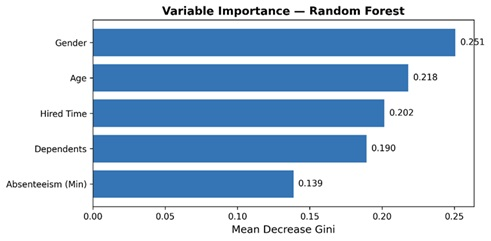
\includegraphics[width=\linewidth]{figures/fig_importance.jpeg}
    \caption{Variable importance (Mean Decrease Gini) for the Random Forest model. Gender is the most discriminating variable, followed by Age and Hired Time. Source: Elaborated by the author.}
    \label{fig:importance}
\end{figure}

\textbf{Gender} emerges as the most discriminating predictor (Gini = 0.252), 
which reflects the strong gender-based stratification observed in the Phase~1 
clustering solution: Clusters 3, 6, and 7 are entirely female (100\%) while 
Clusters 2, 4, and 8 are entirely male (0\% female), making Gender a single 
binary split that immediately separates six of the eight clusters into two 
disjoint sets. From an information-theoretic perspective, this is a 
maximally efficient predictor for early tree splits, which is why it 
dominates the Gini ranking. However, this finding requires careful 
interpretation: Gender's high importance does \textbf{not} mean that gender 
\textit{causes} the observed clustering - it means that the clustering 
algorithm (K-Means in Phase~1) happened to produce clusters that are 
strongly gender-aligned, which in turn makes Gender a highly predictive 
feature for any classifier learning to reconstruct those cluster boundaries. 
The substantive interpretation lies in Phase~1's findings, not in the 
classifier's variable importance.

\textbf{Age} (Gini = 0.218) and \textbf{Hired Time} (Gini = 0.202) form the 
second tier of importance and are nearly equivalent in their predictive 
contribution. This near-parity is consistent with the moderate correlation 
between these two variables ($r = 0.413$; \cref{tab:correlation}): in a 
Random Forest, when two variables share predictive information, the ensemble 
distributes splits between them across different trees, producing similar 
importance scores. The combined importance of Age and Hired Time (0.420) exceeds 
Gender's individual importance, indicating that career-stage 
differentiation - captured jointly by these two variables - is the most 
substantively meaningful axis of cluster separation, even though Gender 
provides the single most efficient split.

\textbf{Absenteeism} occupies the bottom of the ranking (Gini = 0.139) 
despite being the defining characteristic of the outlier Cluster 5 (mean 
1,327 hours versus 99--260 hours for other clusters). This apparent paradox 
illustrates an important property of impurity-based importance measures: 
they reward features that produce \textit{many useful splits across many 
observations}, not features that perfectly identify rare cases. Cluster 5's 
$n=15$ employees represent only 4.5\% of the dataset, so a split on 
Absenteeism - though decisive for these specific cases - contributes 
little to overall impurity reduction. This is precisely why Random Forest 
underperforms on Cluster 5 specifically (recall = 0.400; 
\cref{tab:per_class_rf}): the variable that would correctly identify it is 
systematically de-prioritized by the ensemble's optimization criterion. 
\textbf{Dependents} ranks even lower (Gini below Absenteeism, visible in 
\cref{fig:importance}), but in this case the low importance reflects genuine 
weak predictive value rather than a minority-class blind spot. From an 
ethical and managerial perspective, the prominence of Gender as the top 
predictor warrants explicit acknowledgment and governance, a point developed 
in \cref{sec:discussion}.

\subsection{Statistical Hypothesis Tests}

\subsubsection{Cochran's Q Test (Omnibus)}

\begin{table}[ht]
    \centering
    \begin{threeparttable}
    \caption{Cochran's Q Test}
    \label{tab:cochran}
    \begin{tabular}{lc}
        \toprule
        Statistic & Value \\
        \midrule
        Q         & 175.97 \\
        df        & 3 \\
        p-value   & $<$ 0.001 \\
        Decision  & Reject $H_0$ - models differ significantly \\
        \bottomrule
    \end{tabular}
    \begin{tablenotes}
        \footnotesize
        \item Source: Elaborated by the author.
    \end{tablenotes}
    \end{threeparttable}
\end{table}

\cref{tab:cochran} reports the Cochran's Q test, an omnibus test of whether 
all four models produce equivalent error patterns on the same test set 
\citep{Cochran1950}. The observed Q = 175.97 ($df = 3$, $p < 0.001$) exceeds 
the critical value $\chi^2_{3, 0.95} = 7.81$ by a factor of more than 22, 
unambiguously rejecting equivalence. The magnitude reflects the bimodal 
landscape already evident in \cref{tab:cv_metrics}: the gap between the top 
three models (accuracy $\geq 0.94$) and KNN (0.28) is wide enough for any 
reasonable omnibus test to detect it. This rejection \textbf{authorizes} the 
pairwise comparisons in \cref{tab:mcnemar,tab:ttests} but is silent on 
which pairs differ - hence the McNemar's tests below, with Bonferroni 
correction to control the family-wise error rate across the six 
comparisons.

\subsubsection{McNemar's Tests (Pairwise)}

\begin{table*}[ht]
    \centering
    \begin{threeparttable}
    \caption{Pairwise McNemar's Tests (Bonferroni-corrected $\alpha = 0.0083$)}
    \label{tab:mcnemar}
    \begin{tabular}{llcccccc}
        \toprule
        Model A & Model B & b (A\checkmark\,B$\times$) & c (A$\times$\,B\checkmark) & $\chi^2$ & p-value & Sig. \\
        \midrule
        Multin. Log. Reg. & Decision Tree   & 5 & 3 & 0.50   & 0.480     & ns \\
        Multin. Log. Reg. & Random Forest   & 3 & 3 & 0.00   & 1.000     & ns \\
        Multin. Log. Reg. & KNN ($k=13$)    & 7 & 0 & 165.13 & $<$ 0.001 & *** \\
        Decision Tree     & Random Forest   & 3 & 5 & 0.50   & 0.480     & ns \\
        Decision Tree     & KNN ($k=13$)    & 6 & 9 & 261.35 & $<$ 0.001 & *** \\
        Random Forest     & KNN ($k=13$)    & 7 & 2 & 361.65 & $<$ 0.001 & *** \\
        \bottomrule
    \end{tabular}
    \begin{tablenotes}
        \footnotesize
        \item Source: Elaborated by the author. $b$ = instances correctly classified by A but not B; $c$ = reverse.
        \item Significance: *** $p < 0.001$; ns = not significant after Bonferroni correction.
    \end{tablenotes}
    \end{threeparttable}
\end{table*}

\cref{tab:mcnemar} decomposes the omnibus rejection into specific pairwise 
comparisons. McNemar's test compares the \textbf{discordant predictions} 
between two models on the same test set ($b$: A correct, B wrong; $c$: 
reverse). When $b$ and $c$ are balanced, models are equivalent regardless of 
mean accuracy; substantial divergence indicates one model is systematically 
superior on disagreement cases.

The six pairwise results divide cleanly. The three top-tier comparisons 
(LR vs. DT, LR vs. RF, DT vs. RF) all return non-significant results 
($p = 0.480$, $p = 1.000$, $p = 0.480$) after Bonferroni correction. The 
LR vs. RF case is illustrative: $b = c = 3$ yields $\chi^2 = 0.00$, 
$p = 1.000$ - perfectly symmetric discordance, statistical equivalence in 
its strongest form. The three KNN-related comparisons, by contrast, all 
yield $p < 0.001$ with $\chi^2$ values of 165.13, 261.35, and 361.65 - 
exceeding the Bonferroni-corrected critical value by factors of 20 to 43. 
Particularly striking is LR vs. KNN with $b = 7$, $c = 0$: \textit{zero} 
cases where KNN succeeds and LR fails.

The Bonferroni correction ($\alpha_{corrected} = 0.05/6 = 0.0083$) is 
conservative but the results are robust to it: non-significant cases are 
all $p \geq 0.48$, while significant cases are all $p < 0.001$. From a 
deployment perspective, \cref{tab:mcnemar} establishes empirical grounds 
for model selection on \textbf{secondary criteria} (interpretability, 
variable importance, computational simplicity), since the top three models 
are statistically indistinguishable.

\subsubsection{Corrected Paired t-Tests on CV Folds}

\begin{table*}[h]
    \centering
    \begin{threeparttable}
    \caption{Paired t-Tests (Nadeau \& Bengio Correction)}
    \label{tab:ttests}
    \begin{tabular}{llccccc}
        \toprule
        Model A & Model B & Mean Diff. & $t$ & p-value & Sig. \\
        \midrule
        Multin. Log. Reg. & Decision Tree  & $+0.090$ & 3.03    & 0.014     & ns \\
        Multin. Log. Reg. & Random Forest  & $+0.039$ & 1.64    & 0.136     & ns \\
        Multin. Log. Reg. & KNN ($k=13$)   & $+0.649$ & 11.63   & $<$ 0.001 & *** \\
        Decision Tree     & Random Forest  & $-0.051$ & $-1.69$ & 0.126     & ns \\
        Decision Tree     & KNN ($k=13$)   & $+0.559$ & 10.51   & $<$ 0.001 & *** \\
        Random Forest     & KNN ($k=13$)   & $+0.610$ & 13.12   & $<$ 0.001 & *** \\
        \bottomrule
    \end{tabular}
    \begin{tablenotes}
        \footnotesize
        \item Source: Elaborated by the author. \cite{Nadeau2003} variance correction applied. Bonferroni-corrected $\alpha = 0.0083$.
    \end{tablenotes}
    \end{threeparttable}
\end{table*}

\cref{tab:ttests} complements the McNemar analysis (\cref{tab:mcnemar}) by 
operating on a different data representation: while McNemar compares 
discordant predictions on the held-out test set, the paired t-test compares 
mean accuracy across CV folds. The \cite{Nadeau2003} variance correction is 
applied to address a known statistical problem: in standard CV, training 
sets across folds share approximately 90\% of their observations, violating 
the independence assumption of conventional paired t-tests and inflating 
Type I error rates. The correction adjusts the variance estimate by the 
test-to-training ratio, yielding more conservative and methodologically 
defensible significance estimates.

The results produce the same categorical split as McNemar's tests. The 
three KNN-related comparisons yield massive $t$-statistics (11.63, 10.51, 
13.12) with mean accuracy differences of 0.649, 0.559, and 0.610 - effect 
sizes approaching the full range of accuracy and well below the Bonferroni 
threshold. The three top-tier comparisons all fall above the threshold and 
are non-significant. A nuance worth noting: LR vs. DT ($t = 3.03$, raw 
$p = 0.014$, mean diff $+0.090$) would be significant under uncorrected 
$\alpha = 0.05$. The Bonferroni correction moves it to non-significant, 
which is the methodologically appropriate conclusion - LR shows a 
suggestive but not confirmed advantage over DT.

The convergence between \cref{tab:ttests} and \cref{tab:mcnemar}, despite 
their different statistical machinery (parametric mean comparison vs. 
binomial discordance test), provides \textbf{methodological triangulation} 
that strengthens the validity of the model comparison. The combined 
multi-layered protocol (point estimates with CIs, omnibus test, pairwise 
discordance, and CV-fold parametric tests) is rarely applied in published 
People Analytics studies and constitutes one of the methodological 
contributions of this work.

\subsection{KNN Optimization}
\label{sec:knn_optimization}

\cref{fig:knn_k} presents systematic hyperparameter optimization for KNN, 
ruling out the possibility that its poor performance is an artifact of 
suboptimal $k$ rather than a fundamental model-data mismatch. The curve 
fluctuates narrowly across $k = 1$ to $20$, never exceeding approximately 
0.30. Confidence intervals across different $k$ values \textbf{overlap 
substantially} - no specific $k$ produces a statistically meaningful 
advantage. This is the diagnostic signature of a \textbf{ceiling effect}: 
the model has reached its intrinsic performance limit on this data.

The substantive interpretation is \textbf{geometric incompatibility}. KNN 
assumes class membership clusters in dense feature-space neighborhoods, but 
the ApexBrasil clusters have heterogeneous internal densities and unequal 
sizes ($n = 15$ to $n = 77$). Near boundaries between small and large 
clusters, the 13 nearest neighbors are dominated by the larger cluster 
regardless of true membership. Smaller $k$ values reduce this majority bias 
but introduce variance (wider CIs visible in \cref{fig:knn_k}); larger $k$ 
values amplify the bias without compensating gains. The flat curve thus 
exposes a bias-variance tradeoff that no neighborhood size can resolve. 
For organizations with limited analytical maturity, this distinction 
between tuning failures and inductive bias mismatch is operationally 
important: it prevents wasted effort on hyperparameter search for 
structurally unsuitable models.

\begin{figure}[bt!]
    \centering
    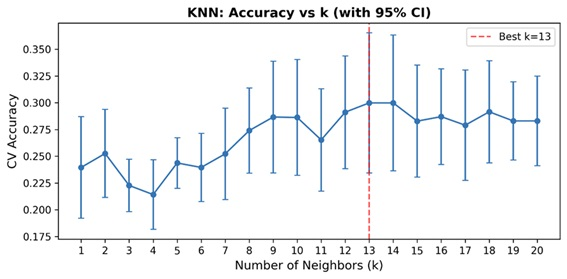
\includegraphics[width=\linewidth]{figures/fig_knn_k.jpeg}
    \caption{KNN cross-validation accuracy as a function of $k$ (number of neighbors), with 95\% confidence intervals. Optimal $k=13$ (accuracy = 0.30). Source: Elaborated by the author.}
    \label{fig:knn_k}
\end{figure}


\section{Discussion}
\label{sec:discussion}

\subsection{Interpretation and Model Comparison}

Multinomial Logistic Regression and Random Forest both achieved test accuracy 
of 0.96, with no statistically significant difference between them or against 
Decision Tree (McNemar $p \geq 0.48$; paired t-test $p \geq 0.126$). As 
discussed in \cref{sec:why_high}, this high performance is methodologically 
expected since the target variable was generated by K-Means from the same 
feature space used as predictors. The supervised models are therefore learning 
to approximate the K-Means decision boundaries, with two important 
implications: (i) the predictability of cluster membership validates the 
Phase~1 segmentation as well-defined, separable groups rather than algorithmic 
artifacts; and (ii) automated assignment of new hires to workforce profiles is 
operationally feasible using only standard ERP data.

Multinomial LR's leading position (CV accuracy 0.9487) suggests that the 
K-Means cluster boundaries are approximately linear in the feature space, 
consistent with K-Means' Euclidean centroid partitioning \citep{Lloyd1982}. 
Its interpretability is an additional advantage for organizational adoption 
in low analytical maturity contexts. Random Forest matches it on the test set 
(0.9604) while offering variable importance rankings (\cref{fig:importance}). 
Decision Tree's unexpectedly strong test accuracy (0.9406) shows that even a 
single tree captures most of the cluster structure, though its higher fold 
variance (SE = 0.019 vs. 0.014 for LR) signals less stable generalization. 
KNN's failure (accuracy 0.28) - confirmed by Cochran's Q ($Q = 175.97$, 
$p < 0.001$) and the pairwise tests - is structural: when cluster boundaries 
are well-defined and approximately linear, multiple classification paradigms 
learn them effectively, while distance-based approaches struggle with the 
heterogeneous cluster densities of this dataset \citep{Duda2001}.

\subsection{Comparison with Literature}
The comparative pattern observed is consistent with findings from \cite{Alsaadi2022}, who reported similar accuracy hierarchies in HR classification tasks. \cite{Fallucchi2020} also demonstrated that ensemble methods achieve strong performance in employee-related prediction. The distinctive contribution of this study lies in the sequential clustering~$\rightarrow$~classification approach with rigorous statistical validation, which is absent in prior HR classification literature.

\subsection{Practical Implications}
The classification models enable three operational capabilities for ApexBrasil:

\begin{itemize}
    \item \textbf{Automated onboarding classification}: New employees can be assigned to a workforce profile at hiring, based on their age, Hired Time, gender, dependents, and projected absenteeism. This enables immediate personalized onboarding.
    \item \textbf{Dynamic profile monitoring}: As employee attributes change over time, the classification model can detect profile transitions, supporting proactive people management interventions.
    \item \textbf{HR policy differentiation}: The eight profiles provide a structured basis for differentiated policies in compensation, career development, absenteeism management, and well-being programs.
\end{itemize}

\subsection{Ethical Considerations}
\label{sec:ethics}

Classification models applied to employee data require careful 
ethical oversight, particularly when sensitive attributes emerge as 
strong predictors. The prominence of Gender as the top discriminating 
variable in this study (Gini = 0.252; \cref{fig:importance}) 
demands explicit acknowledgment: while Gender is analytically 
significant for predicting cluster membership, the resulting profiles 
must inform , not determine , HR decisions \citep{Tursunbayeva2022}. 
The distinction is consequential. Allowing predicted cluster 
membership to drive consequential HR actions (promotion shortlisting, 
training allocation, performance review prioritization) would 
operationalize a feedback loop in which gender-segregated profiles 
become self-reinforcing through algorithmic recommendation, 
amplifying rather than mitigating existing workforce asymmetries.

This concern is not abstract in the Brazilian public-sector context. 
The General Data Protection Law (\textit{Lei Geral de Proteção de 
Dados Pessoais}, LGPD - Lei nº 13.709/2018) explicitly establishes 
\textit{non-discrimination} as a binding principle of personal data 
processing (Art.~6º, IX), prohibiting the use of personal data for 
discriminatory, unlawful, or abusive purposes. Furthermore, 
employee gender qualifies as \textit{sensitive personal data} under 
the LGPD's broader interpretation when processed in contexts that 
may produce discriminatory effects (Art.~5º, II, in conjunction with 
Art.~11). Although the present study uses Gender exclusively as an 
analytical variable to characterize pre-existing workforce 
heterogeneity , and not as a basis for individual decisions , 
any operational deployment of the classification models must 
incorporate explicit safeguards against discriminatory downstream 
use. This is consistent with the framework proposed by the 
\textit{Autoridade Nacional de Proteção de Dados} (ANPD) in 
Resolution CD/ANPD nº 4/2023 on the rights of data subjects, which 
establishes that automated decisions affecting employment status 
warrant heightened transparency and human review obligations.

A defensible operational deployment of the present classification 
models therefore requires a layered governance architecture aligned 
with Privacy by Design principles \citep{Cavoukian2009}. First, 
\textbf{purpose limitation}: cluster predictions should be confined 
to operational personalization (e.g., onboarding workflow design, 
proactive identification of well-being intervention needs) and 
explicitly excluded from consequential decisions such as 
performance evaluation, compensation, promotion, or dismissal. 
Second, \textbf{human-in-the-loop oversight}: all HR actions 
informed by cluster membership should require explicit human 
review, with the predicted profile serving as one input among 
several rather than as a deterministic recommendation. Third, 
\textbf{disparate impact monitoring}: periodic audits should 
compare HR outcomes (training participation, internal mobility, 
attrition rates) across the eight profiles to detect any 
systematic disparities that might indicate algorithmic 
discrimination, even when no individual decision was explicitly 
gender-based. Fourth, \textbf{data subject rights}: employees 
should be informed about the existence of the segmentation, the 
purposes for which it is used, and their LGPD rights to access 
their cluster assignment (Art.~18, II), to request review of 
automated decisions affecting them (Art.~20), and to oppose 
processing that violates the law (Art.~18, §2º).

Beyond compliance, an ethical deployment requires reflection on 
the substantive composition of the cluster solution itself. The 
fact that K-Means produced six of eight clusters with 0\% or 100\% 
female composition (\cref{tab:distribution}) is not an artifact of 
the algorithm , it reflects pre-existing gender-based 
stratification in ApexBrasil's workforce, particularly the 
clustering of women in profiles characterized by higher 
absenteeism (Clusters 3, 5) and the absence of women from 
profiles characterized by high tenure with low dependents 
(Cluster 2). These patterns may themselves warrant organizational 
attention as potential indicators of structural inequalities in 
career trajectories, work-life balance support, or retention 
dynamics. The classification model, in this sense, is both a 
practical tool for differentiated HR policy and a diagnostic 
instrument that surfaces structural patterns deserving 
substantive HR intervention , not algorithmic 
self-reinforcement. The ethical posture proposed here aligns 
with the emerging consensus in People Analytics scholarship that 
positions algorithmic systems as decision-support rather than 
decision-making tools \citep{Tursunbayeva2022,Polzer2022}, with 
particular care required in public-sector contexts where 
employment decisions are subject to constitutional principles of 
impessoalidade and equality (Constituição Federal de 1988, 
Art.~37).


\section{Conclusions}
\label{sec:conclusions}

\subsection{Synthesis of Findings}
This study (Phase~2) evaluated four supervised classification models for predicting employee membership in eight workforce profiles previously identified through K-Means clustering (Phase~1) at ApexBrasil.

Multinomial Logistic Regression (test accuracy: 0.96; CV: 0.95, 95\% CI: [0.917, 0.980]) and Random Forest (test accuracy: 0.96; CV: 0.91, 95\% CI: [0.876, 0.945]) achieved near-perfect classification, both validated by rigorous 10-fold CV and statistical hypothesis testing. Cochran's Q test ($Q = 175.97$, $p < 0.001$) confirmed significant overall model differences, while pairwise McNemar's tests showed no significant difference among the top three models - only KNN was significantly inferior.

\subsection{Scientific Contributions}
\begin{itemize}
    \item \textbf{Theoretical}: Validates the sequential CRISP-DM approach (clustering~$\rightarrow$~classification) for People Analytics by framing the supervised stage as \textit{internal validation of the geometric separability} of the Phase~1 profiles, rather than as external predictive assessment. The high accuracy achieved confirms that the eight profiles occupy distinct regions of the feature space and that their boundaries are learnable by alternative classifiers, bridging exploratory segmentation and operational deployment while maintaining epistemological rigor about what the sequential design can and cannot claim.
    \item \textbf{Methodological}: Provides a replicable protocol with rigorous statistical validation - 10-fold CV, 95\% confidence intervals, Cochran's Q omnibus test, McNemar's pairwise tests with Bonferroni correction, and Nadeau-Bengio corrected paired t-tests - establishing a benchmark for evaluating classification techniques on clustering-derived labels in HR datasets.
    \item \textbf{Practical}: Demonstrates that automated employee classification is achievable with open-source tools (Python/scikit-learn), standard ERP data, and models interpretable by non-technical managers - reinforcing People Analytics feasibility in low analytical maturity contexts. Therefore, the objective is not external predictive generalization but internal validation of segmentation consistency and operational deployability.
\end{itemize}

\subsection{Limitations}
\begin{itemize}
    \item \textbf{Single case}: Results refer specifically to ApexBrasil's workforce structure in a federal public-sector context. The study is therefore best read as a \textit{proof-of-concept of the CRISP-DM clustering~$\rightarrow$~classification protocol} rather than as evidence that the eight profiles generalize to other organizations. The framework and statistical protocol are transferable; multi-case replications across other Brazilian public organizations are needed for external validation.
    \item \textbf{Circular target variable}: The target variable derives from the same features used as predictors, which inherently facilitates high accuracy. While acknowledged as a validation mechanism, independent external labels (e.g., HR expert classifications) would strengthen the methodology.
    \item \textbf{Limited variables}: Administrative data do not include behavioral variables (engagement, satisfaction) or performance metrics. Future studies should integrate complementary data sources.
    \item \textbf{Cross-sectional design and model decay}: Classification was trained on a snapshot at December 31, 2023. As workforce attributes evolve over time (aging, tenure accumulation, dependents changes, absenteeism dynamics), model decay is expected and the classifier should be periodically re-evaluated and retrained. This is not merely a statistical concern but an operational and ethical requirement under the governance framework in \cref{sec:ethics}, which anticipates human-in-the-loop monitoring at deployment.
    \item \textbf{Sample size and minority-class stability}: With $n=335$ distributed across 8 classes, minority clusters (notably Cluster~5 with $n=15$ total and $n=5$ in the held-out test set) carry limited statistical power for per-class metric estimation. Confidence intervals around per-class recall and precision are correspondingly wide, and conclusions about minority-cluster classification quality should be treated as directional rather than definitive. Replication with larger multi-organizational samples would be required to establish per-cluster performance with narrower uncertainty.
\end{itemize}

\subsection{Directions for Future Research}
\begin{itemize}
    \item \textbf{External validation}: Replicate the clustering~$\rightarrow$~classification framework in other Brazilian public organizations to assess the transferability of both the methodological protocol and the profile taxonomy.
    \item \textbf{Temporal monitoring}: Conduct longitudinal studies tracking classifier performance over time to quantify model decay, establish evidence-based retraining schedules, and support the human-in-the-loop monitoring obligations implied by LGPD Art.~20 (right to explanation and review of automated decisions).
    \item \textbf{Data enrichment}: Integrate engagement surveys, performance evaluations, and qualitative interviews to move beyond the demographic-and-absenteeism feature space of the present study.
    \item \textbf{Advanced models}: Evaluate gradient boosting (XGBoost, LightGBM) and neural networks, particularly for minority-class improvement.
\end{itemize}


\section*{Reproducibility}

All analyses are fully reproducible. The complete Python code, dataset specifications, and parameter configurations are documented below.

Experimental Parameters
\begin{enumerate}
    \item Random seed: 123
    \item K-Means clusters: 8 (\texttt{n\_init=25})
    \item Cross-validation: 10-fold stratified
    \item Train/Test split: 70/30 stratified
    \item Confidence level: 95\% ($t$-distribution, $df=9$)
    \item Multinomial LR: solver = \texttt{newton-cg}, \texttt{max\_iter=10000}
    \item Random Forest: \texttt{n\_estimators=500}
    \item KNN: best $k=13$ (grid search $k=1..20$)
    \item Bonferroni $\alpha$: $0.05/6 = 0.0083$
\end{enumerate}

\textbf{Software}: Python 3.12, scikit-learn 1.8.0, scipy 1.14, pandas 3.0, matplotlib 3.9, seaborn 0.13.

\textbf{Code repository}: The complete analysis script is available as supplementary material -  \url{https://github.com/ciuffciuff/Phase2_article/blob/main/Classification_Phase2_Statistical.py}


\section*{Acknowledgments}

The author acknowledges ApexBrasil for institutional support and the PPCA/UnB program for the research framework that made this study possible.


%% Specify your .bib file name here, without the extension .bib
\bibliography{references}

\end{document}
